\documentclass[12pt,a4paper]{article}

% --------------------
% Packages
% --------------------
\usepackage[top=2.5cm,bottom=2.5cm,left=2.7cm,right=2.7cm]{geometry}
\usepackage{amsmath,amssymb}
\usepackage{graphicx}
\usepackage{booktabs}
\usepackage{setspace}
\usepackage{indentfirst}
\usepackage{titlesec}
\usepackage{xcolor}
\usepackage{array}

% hyperref should be loaded before xepersian in many cases
\usepackage[colorlinks=true,linkcolor=blue,citecolor=blue,urlcolor=blue]{hyperref}

\usepackage{xepersian}

% --------------------
% Fonts
% --------------------
\settextfont{Vazirmatn}
\setdigitfont{Vazirmatn}
\setlatintextfont{Times New Roman}

% --------------------
% Layout settings
% --------------------
\setstretch{1.35}          % line spacing
\setlength{\parskip}{0.4em} % space between paragraphs
\setlength{\parindent}{1.2cm}

% --------------------
% Section formatting
% --------------------
\titleformat{\section}
{\Large\bfseries}
{\thesection}
{0.8em}
{}

\titleformat{\subsection}
{\large\bfseries}
{\thesubsection}
{0.8em}
{}

\begin{document}
	
\begin{titlepage}
	\centering
	
	% فاصله از بالای صفحه
	\vspace*{2cm}
	
	% عنوان اصلی
	{\Huge\bfseries گزارش کار فنی پروژه\par}
	\vspace{0.6cm}
	
	% نام پروژه با لینک گیت‌هاب
	{\LARGE\bfseries 
		\href{https://github.com/alitkbbl/PhysioStress}{\textcolor{blue}{\lr{PhysioStress}}}
		\par}
	
	% زیرعنوان انگلیسی (در صورت نیاز)
	\vspace{0.5cm}
	{\large\itshape Technical Report\par}
	
	% خط افقی تزئینی
	\vspace{0.8cm}
	\rule{\linewidth}{0.4pt}
	\vspace{0.8cm}
	
	% نام نویسنده
	{\Large علی تقی‌زاده\par}
	\vspace{0.3cm}
	
	% وابستگی
	{\large دانشکدهٔ علوم کامپیوتر، دانشگاه صنعتی امیرکبیر\par}
	% اگر دوست داری همین متن قبلی‌ات بماند:
	% {\large دانشکده علوم کامپیوتر امیرکبیر\par}
	
	% فاصله‌ی انعطاف‌پذیر برای بالانس صفحه
	\vfill
	


	
	% فاصله از پایین صفحه
	\vspace*{1.5cm}
\end{titlepage}

	
	\tableofcontents
	\newpage

	\section{پیش‌زمینه (\lr{Background})}
	
	\subsection{چرا سیگنال‌های فیزیولوژیک استرس را نشان می‌دهند؟}
	
	سیستم عصبی خودمختار (\lr{ANS}) دارای دو شاخه است که به‌طور پیوسته و غیرارادی بدن را تنظیم می‌کنند: شاخه \textbf{سمپاتیک} («مبارزه یا فرار»، که در اثر تهدید یا تلاش فعال می‌شود) و شاخه \textbf{پاراسمپاتیک} («استراحت و هضم»، که در حالت آرامش غالب است). استرس روانی حاد باعث ایجاد یک موج سمپاتیک با نشانه‌های فیزیولوژیک چندسیستمی و قابل‌تشخیص می‌شود:
	

\begin{itemize}
    \item \textbf{افزایش ضربان قلب و کاهش تغییرپذیری ضربان قلب (\lr{HRV}):} یک قلب آرام مانند مترونوم نمی‌تپد؛ بلکه با هر نفس تند و کند می‌شود (که بیشتر توسط عصب واگ کنترل می‌شود). فعال‌شدن سیستم سمپاتیک این تغییرپذیریِ وابسته به واگ را سرکوب می‌کند؛ بنابراین، \lr{HRV} پایین در کنار ضربان قلب بالا یکی از تکرارپذیرترین نشانگرهای استرس در ادبیات سایکوفیزیولوژی است.
    \item \textbf{افزایش هدایت پوستی:} غدد عرق در پوست (به‌ویژه در کف دست، مچ و انگشتان) تقریباً منحصراً توسط اعصاب سمپاتیک تحریک می‌شوند، که فعالیت الکترودرمال (\lr{EDA}) را به یکی از معدود سیگنال‌های محیطی با ارتباط تقریباً مستقیم با برانگیختگی سمپاتیک تبدیل می‌کند. \lr{EDA} دارای یک سطح پایه با حرکت کند (مؤلفه \textbf{تونیک} یا سطح هدایت پوستی) و برجستگی‌های سریع و گسسته (پاسخ‌های \textbf{فازیک} هدایت پوستی، \lr{SCRs}) است که با رویدادهای برانگیزاننده همگام هستند.
    \item \textbf{تنفس سریع‌تر و کم‌عمق‌تر می‌شود:} آماده‌سازی بدن برای واکنش، سرعت تنفس را افزایش و هم‌زمان عمق هر نفس را کاهش می‌دهد.
    \item \textbf{انقباض عضلانی:} سفت‌کردن بدن، فشردن فک و تنش وضعیتی عمومی، فعالیت الکترومیوگرافی (\lr{EMG}) را به‌ویژه در بالاتنه افزایش می‌دهد.
    \item \textbf{کاهش دمای محیطی پوست:} خون از پوست به سمت عضلات بزرگ و مرکز بدن هدایت می‌شود (تنگی عروق) که همان حس آشنای «دست‌های سرد» را ایجاد می‌کند.
    \item \textbf{تغییر الگوهای حرکتی:} بی‌قراری در شرایط استرس‌زا و حرکات ناشی از ژست‌گرفتن/خندیدن در هنگام سرگرمی، هر دو با بی‌حرکتی در حالت پایه (آرامش) تفاوت دارند.
\end{itemize}

از آنجا که \textit{هر یک از این سیگنال‌ها} توسط گجت‌های پوشیدنی قابل‌اندازه‌گیری است، و از آنجا که حالت سرگرمی (\lr{Amusement} - یک حالت متفاوت با برانگیختگی بالا اما مثبت) نیز چندین مورد از آن‌ها را مختل می‌کند، هدف این پروژه تعیین این است که آیا یک مدل یادگیری ماشین می‌تواند تنها با استفاده از این سیگنال‌های محیطی، استرس را هم از حالت پایه آرام \textbf{و هم} از یک حالت برانگیخته غیر استرس‌زا متمایز کند — که نسخه ۳-کلاسه و واقع‌گرایانه‌تر این مسئله است.

\subsection{چرا این کار دشوار است؟}
دو عامل باعث می‌شود تشخیص استرس مبتنی بر گجت‌های پوشیدنی در عمل دشوار باشد که هر دو در طراحی این پروژه مستقیماً مورد توجه قرار گرفته‌اند:
\begin{enumerate}
    \item \textbf{تفاوت افراد با یکدیگر:} ضربان قلب در حالت استراحت، سطح معمول هدایت پوستی، و اینکه بدن یک فرد چقدر در برابر استرس از خود واکنش نشان می‌دهد («واکنش‌پذیری»)، بین افراد مختلف به دلایلی نامرتبط با سطح استرس فعلی آن‌ها تفاوت زیادی دارد. یک مدل باید بتواند به یک شخص \textit{جدید} که قبلاً ندیده تعمیم یابد، نه اینکه فقط داده‌های ۱۴ نفری که با آن‌ها آموزش دیده است را حفظ کند.
    \item \textbf{هم‌پوشانی استرس با سایر حالت‌های برانگیختگی بالا:} سرگرمی و استرس از چندین جنبه فیزیولوژیک شبیه هم هستند (مثلاً هر دو باعث افزایش ضربان قلب و حرکت می‌شوند)، بنابراین مرز دسته‌بندی واقعاً دشوار، معمولاً بین استرس و سرگرمی است، نه استرس و آرامش.
\end{enumerate}


\section{داده‌ها (\lr{Data})}
مجموعه داده شامل ۱۵ سوژه است که هر کدام به دو دستگاه پوشیدنی مجهز شده‌اند:
\begin{itemize}
    \item \textbf{بند حسگر قفسه سینه:} شامل \lr{ECG}، \lr{EDA}، \lr{EMG}، تنفس، دمای پوست و شتاب‌سنج ۳-محوره که با فرکانس ۱۰۰ هرتز نمونه‌برداری می‌شوند.
    \item \textbf{حسگر مچ‌بند:} شامل پالس حجم خون (\lr{BVP})، \lr{EDA}، دمای پوست و شتاب‌سنج ۳-محوره که با نرخ‌های معمول ساعت‌های هوشمند (\lr{BVP} با نرخ ۶۴ هرتز، \lr{EDA}/دما با نرخ ۴ هرتز، شتاب‌سنج با نرخ ۳۲ هرتز) نمونه‌برداری می‌شوند.
\end{itemize}

روندهای ثبت داده برای هر سوژه در سه شرایط — پایه (آرامش)، استرس و سرگرمی — انجام شده است و سیگنال‌های خام با استفاده از یک مدل مبتنی بر اصول فیزیولوژیک (\lr{\texttt{src/synthetic\_data.py}}) تولید شده‌اند که طوری طراحی شده تا هر شرایط در \textit{جهتی} تغییر کند که فیزیولوژی خودمختار واقعی در آن جهت حرکت می‌کند: ضربان قلب بالاتر و \lr{HRV} پایین‌تر در شرایط استرس، \lr{EDA} افزایش‌یافته در شرایط استرس، تنفس سریع‌تر/کم‌عمق‌تر در شرایط استرس، افت دما ناشی از انقباض عروق در شرایط استرس و غیره.

\vspace{0.5cm}
\noindent\textbf{اهداف طراحی برای یک مسئله طبقه‌بندی واقع‌گرایانه.} دو ویژگی در مدل سیگنال برای معنادار کردن مسئله طبقه‌بندی نهایی حائز اهمیت هستند:
\begin{enumerate}
    \item \textbf{دریفت (رانش) فیزیولوژیک درون‌شرایطی:} هر پارامتر محرک (ضربان قلب لحظه‌ای، \lr{HRV}، و ...) در طول بخش‌های چند دقیقه‌ای مربوط به هر وضعیت، از یک فرآیند بازگشت-به-میانگین پیروی می‌کند، نه اینکه فقط یک عدد ثابت برای کل بازه باشد.
    \item \textbf{واکنش‌پذیری هر فرد:} هر سوژه دارای یک \textit{واکنش‌پذیری} تصادفی مختص خود برای هر سیگنال است (اینکه سیگنال‌های او تحت تأثیر استرس مستقل از سطح پایه چقدر جابجا می‌شود).
\end{enumerate}

سیگنال‌ها به پنجره‌های ۶۰ ثانیه‌ای (با ۵۰٪ هم‌پوشانی) تقسیم شدند و در مجموع \textbf{۴۹۵ پنجره از ۱۵ سوژه} به دست آمد: ۲۲۵ پایه، ۱۶۵ استرس، ۱۰۵ سرگرمی.

\begin{figure}[htbp]
    \centering
    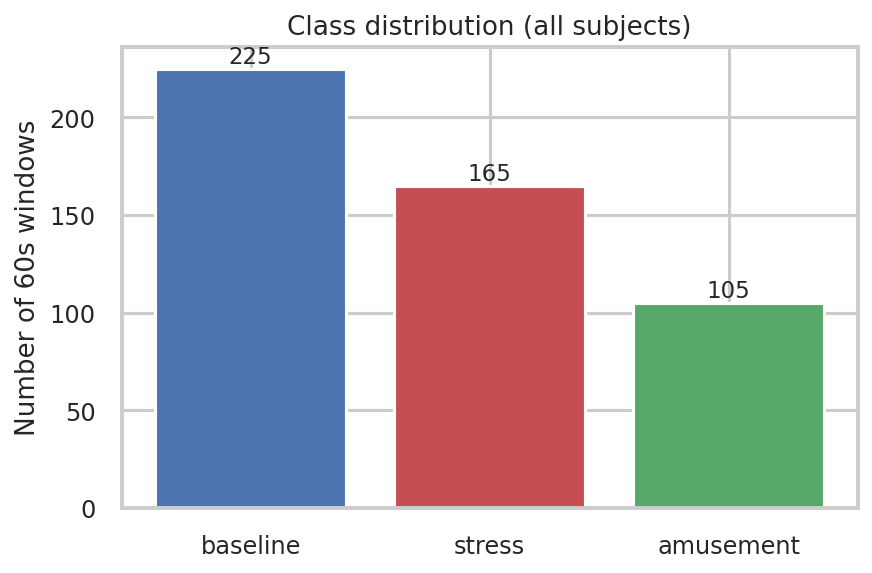
\includegraphics[width=0.7\textwidth]{../results/figures/class_distribution.png}
    \caption{توزیع کلاس‌ها}
\end{figure}

	\newpage
\section{روش‌شناسی (\lr{Methodology})}

\subsection{تحلیل ویژگی‌های استخراج‌شده و مبانی فیزیولوژیک آن‌ها}
به منظور درک دقیق تغییرات حالت‌های فیزیولوژیک و روان‌شناختی (مانند استرس و برانگیختگی)، ویژگی‌های مختلفی از سیگنال‌های زیستی استخراج می‌شوند. در این بخش، به بررسی تفصیلی هر یک از این گروه‌ها، ویژگی‌های کلیدی استخراج‌شده و دلایل فیزیولوژیک پدیدآورنده آن‌ها پرداخته می‌شود:

\paragraph{۱. فعالیت الکترودرمال (\lr{EDA} - ثبت‌شده از قفسه سینه و مچ):}
سیگنال فعالیت الکترودرمال یکی از حساس‌ترین نشانگرهای فعالیت سیستم عصبی سمپاتیک (\lr{SNS}) است. ویژگی‌های استخراج‌شده از این سیگنال عمدتاً به دو بخش تقسیم می‌شوند:
\begin{itemize}
	\item \textbf{ویژگی‌های تونیک (\lr{Tonic} - سطح کند):} شامل میانگین و شیب فعالیت تونیک که نشان‌دهنده تغییرات بلندمدت و تدریجی در رسانایی پوست هستند.
	\item \textbf{ویژگی‌های فازیک (\lr{Phasic} - پاسخ‌های سریع):} شامل انحراف‌معیار مولفه فازیک که تغییرات ناگهانی و کوتاه تغییریافته توسط محرک‌ها را منعکس می‌کند.
\end{itemize}
\textbf{تحلیل فیزیولوژیک:} فعال شدن سیستم عصبی سمپاتیک در پاسخ به استرس یا برانگیختگی عاطفی، منجر به افزایش ترشح غدد عرق اکرین در لایه‌های پوست می‌شود. این فرآیند با افزایش مجراهای رسانا، مقاومت الکتریکی پوست را کاهش و رسانایی آن را افزایش می‌دهد. افزایش سطح عمومی رسانایی (تونیک) به همراه فراوانی و دامنه پاسخ‌های سریع الکترودرمال (فازیک) نشان‌دهنده مستقیم برانگیختگی سمپاتیک است.

\paragraph{۲. تغییرپذیری ضربان قلب (\lr{HRV}):}
تغییرپذیری ضربان قلب نشان‌دهنده تعامل بین شاخه‌های سمپاتیک و پاراسمپاتیک (واگ) سیستم عصبی خودکار (\lr{ANS}) است. شاخص‌های استخراج‌شده عبارتند از:
\begin{itemize}
	\item \textbf{شاخص‌های حوزه زمان:} میانگین ضربان قلب (\lr{HR})، انحراف‌معیار فواصل ضربان‌ها (\lr{SDNN}) و ریشه دوم میانگین مربع تفاضل‌های متوالی (\lr{RMSSD}).
	\item \textbf{شاخص‌های حوزه فرکانس:} نسبت توان فرکانس پایین به فرکانس بالا (\lr{LF/HF}).
\end{itemize}
\textbf{تحلیل فیزیولوژیک:} در شرایط آرامش، عصب واگ (پاراسمپاتیک) فعال است و اثر ترمزکننده بر روی گره سینوسی-دهلیزی دارد که منجر به نوسان و تغییرپذیری بالا در فواصل ضربان‌ها (\lr{HRV} بالا) می‌شود. تحت استرس و فشارهای روانی، اثر تنظیمی واگ کاهش یافته و مسیر سمپاتیک غالب می‌شود. این پدیده باعث یکنواخت شدن فواصل ضربان قلب و در نتیجه کاهش معنی‌دار در شاخص‌های \lr{SDNN} و \lr{RMSSD} می‌گردد. همچنین افزایش نسبت \lr{LF/HF} نشان‌دهنده برهم‌خوردن تعادل سمپاتوواگال به سمت غلبه سمپاتیک است.

\paragraph{۳. الکترومایوگرافی (\lr{EMG}):}
سیگنال الکترومایوگرافی میزان فعالیت الکتریکی ماهیچه‌ها را اندازه‌گیری می‌کند. شاخص‌های آماری و فرکانسی کلیدی استخراج‌شده شامل جذر میانگین مربعات (\lr{RMS})، انحراف‌معیار دامنه سیگنال و نرخ عبور از صفر (\lr{ZC}) هستند.  
\textbf{تحلیل فیزیولوژیک:} در مواجهه با استرس، بدن به صورت ناخودآگاه وارد واکنش «جنگ یا گریز» می‌شود. این پاسخ دفاعی با منقبض شدن عضلات ارادی و غیرارادی (به‌ویژه در نواحی شانه، گردن و صورت) همراه است تا بدن را آماده واکنش فیزیکی کند. افزایش شاخص \lr{RMS} بازتاب‌دهنده افزایش به‌کارگیری واحدهای حرکتی عضلانی و فرکانس شلیک آن‌ها در اثر تنش عصبی است.

\paragraph{۴. تنش و الگوهای تنفسی:}
ویژگی‌های استخراج‌شده شامل نرخ تنفس (تعداد تنفس در دقیقه)، دامنه دم و بازدم و میزان تغییرپذیری در نرخ تنفس است.  
\textbf{تحلیل فیزیولوژیک:} سیستم تنفسی به شدت تحت تأثیر نیازهای متابولیک و وضعیت عاطفی قرار دارد. در شرایط استرس‌زا، تحریک سمپاتیک باعث گشاد شدن برونش‌ها و افزایش نرخ تنفس می‌شود تا اکسیژن‌رسانی به بافت‌ها تسریع گردد. این فرآیند معمولاً منجر به تنفس‌های سریع‌تر، سطحی‌تر (کاهش دامنه موثر) و نامنظم‌تر (کاهش تغییرپذیری کنترل‌شده) می‌شود.

\paragraph{۵. دمای پوست:}
ویژگی‌های استخراج‌شده از حسگرهای دما شامل میانگین دما، شیب تغییرات دما در طول زمان و انحراف‌معیار آن است.  
\textbf{تحلیل فیزیولوژیک:} پاسخ فیزیولوژیک به استرس شامل بازتوزیع جریان خون از بخش‌های محیطی (پوست و اندام‌های انتهایی مانند انگشتان) به سمت ارگان‌های حیاتی و ماهیچه‌های بزرگ است. این پدیده که ناشی از انقباض عروق محیطی (\lr{Vasoconstriction}) به واسطه گیرنده‌های آلفا-آدرنرژیک تحت کنترل سمپاتیک است، باعث افت ناگهانی و ملموس دمای پوست در نقاط محیطی و تغییر در شیب حرارتی می‌شود.

\paragraph{۶. شتاب‌سنج (\lr{Accelerometer}):}
ویژگی‌های استخراج‌شده شامل میانگین و انحراف‌معیار اندازه شتاب کلی در سه محور مختصات و انرژی حرکتی است.  
\textbf{تحلیل فیزیولوژیک:} داده‌های شتاب‌سنج نه تنها برای فیلتر کردن آرتیفکت‌های حرکتی در سایر سیگنال‌ها (مانند حذف نویز حرکت از روی \lr{EDA} و \lr{HRV}) کاربرد دارند، بلکه الگوهای رفتاری مرتبط با استرس را نشان می‌دهند. برای مثال، حرکات بی‌قرار، لرزش‌های خفیف دست یا بی‌حرکتی ناشی از تمرکز شدید یا انجماد تنش‌زا، الگوهای انرژی و انحراف‌معیار متفاوتی را در شتاب‌سنج ثبت می‌کنند که به تمایز حالت‌های شناختی کمک می‌کند.



	\newpage
\section{نتایج (\lr{Results})}

\subsection{Model Comparison}
\begin{table}[htbp]
	\centering
	\begin{latin} % شروع محیط انگلیسی برای جدول
		\begin{tabular}{lccc}
			\toprule
			\textbf{Model} & \textbf{Accuracy} & \textbf{Macro F1-Score} & \textbf{LOSO Accuracy Std} \\
			\midrule
			\textbf{Gradient Boosting (HistGB)} & \textbf{0.891} & \textbf{0.862} & 0.067 \\
			Random Forest & 0.875 & 0.839 & 0.096 \\
			Logistic Regression & 0.853 & 0.810 & 0.097 \\
			SVM (RBF) & 0.804 & 0.745 & 0.110 \\
			Baseline (Majority Class) & 0.455 & 0.208 & 0.000 \\
			\bottomrule
		\end{tabular}
	\end{latin} % پایان محیط انگلیسی
	\caption{Performance comparison of various models across 15 subjects.}
\end{table}


\begin{figure}[htbp]
    \centering
    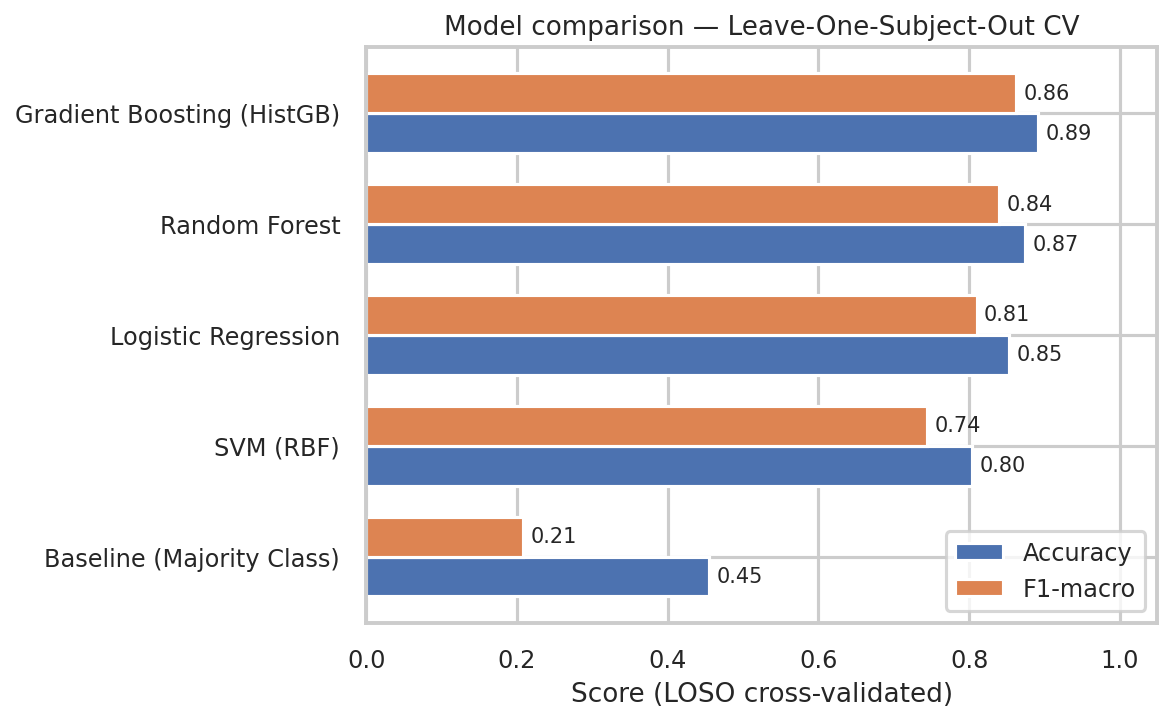
\includegraphics[width=0.8\textwidth]{../results/figures/model_comparison.png}
    \caption{مقایسه مدل‌ها}
\end{figure}

تمامی مدل‌های واقعی عملکرد بسیار بهتری نسبت به خط پایه دارند. متدهای مبتنی بر درخت (گرادیان بوستینگ و جنگل تصادفی) از متدهای خطی و هسته‌ای بهتر عمل می‌کنند که نشان‌دهنده رابطه غیرخطی و آستانه‌ای ویژگی‌ها با هدف است (مثلاً ویژگی حرکت که در حالت استراحت صفر است و با شروع حرکت ناگهان پرش می‌کند).

\subsection{ماتریس درهم‌ریختگی (بهترین مدل، تجمیع شده در تمام ۱۵ فولد \lr{LOSO})}

\begin{figure}[htbp]
    \centering
    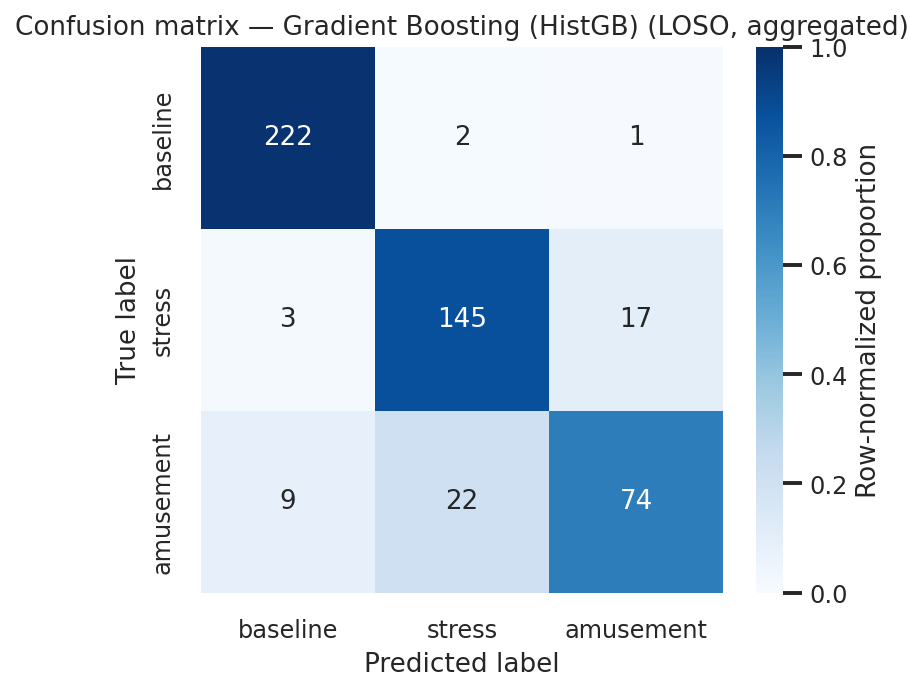
\includegraphics[width=0.7\textwidth]{../results/figures/confusion_matrix_best_model.png}
    \caption{ماتریس درهم‌ریختگی بهترین مدل}
\end{figure}


\textbf{حالت پایه تقریباً بی‌نقص طبقه‌بندی شده است} (۲۲۲ از ۲۲۵، یعنی فراخوانی ۹۸.۷٪) — این حالت از نظر فیزیولوژیک «ساکت» است و تمایز آن آسان است. خطای غالب مربوط به \textbf{اشتباه گرفتن استرس و سرگرمی} است (۱۷ نمونه استرس به جای سرگرمی و ۲۲ نمونه سرگرمی به جای استرس پیش‌بینی شده‌اند). این دقیقاً مطابق با اصول فیزیولوژی است: هر دو حالت دارای برانگیختگی بالای سمپاتیک هستند و مرز بین آن‌ها ذاتاً سخت‌ترین مرز برای تفکیک است.

\subsection{واریانس \lr{LOSO} بین سوژه‌ها}
دقت مدل بهترین (گرادیان بوستینگ) روی افراد کنار گذاشته شده تفاوت‌های معناداری دارد:

\begin{figure}[htbp]
    \centering
    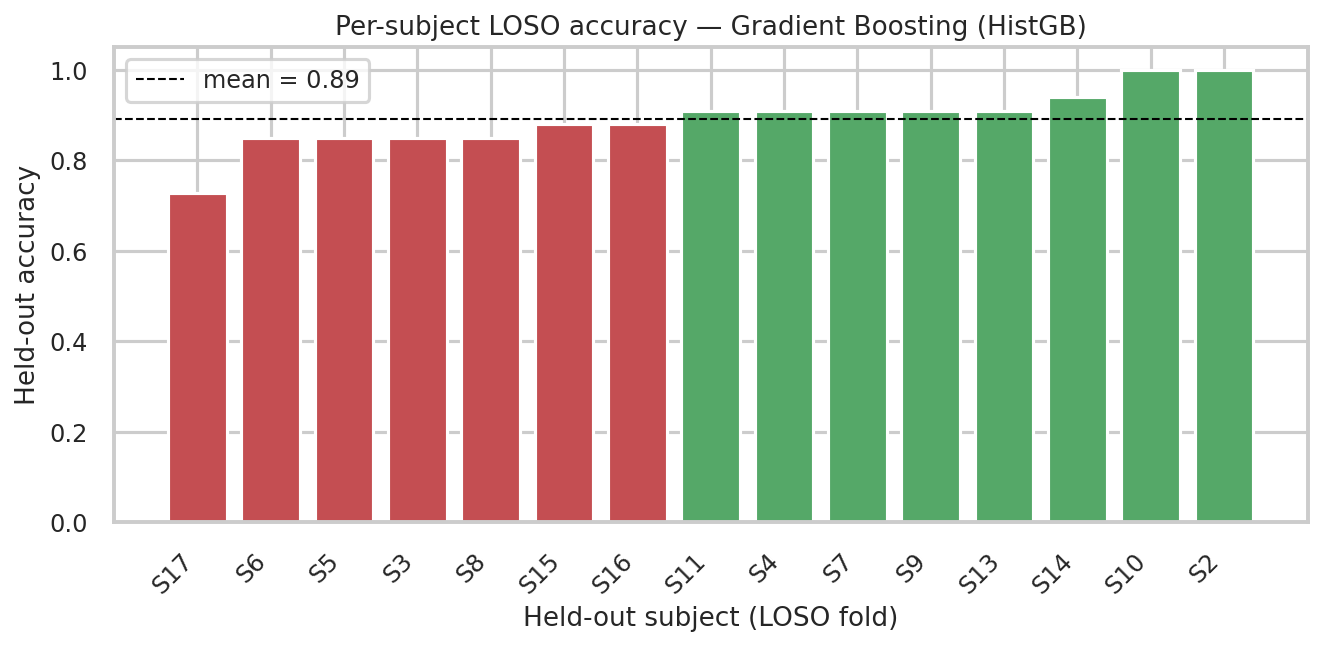
\includegraphics[width=0.8\textwidth]{../results/figures/loso_per_subject_accuracy.png}
    \caption{دقت مدل برای هر سوژه (\lr{LOSO})}
\end{figure}

سوژه \lr{S17} (سخت‌ترین) با دقت ۰.۷۲۷، چندین سوژه بین ۰.۸۴۸ تا ۰.۹۳۹، و سوژه‌های \lr{S2, S10} با دقت بی‌نقص ۱.۰۰۰.
میانگین کل ۰.۸۹۱ با انحراف معیار ۰.۰۶۷ است — یک پراکندگی واقعی که نشان می‌دهد \textbf{تعمیم دادن مدل به افراد جدید، برای برخی افراد بسیار سخت‌تر از دیگران است}.

\subsection{تکرار مستقل و بررسی حذف نرمال‌سازی (نوت‌بوک ۰۳)}
بررسی‌ها در یک پیاده‌سازی مستقل (\lr{Notebook 03}) نشان داد که آیا نرمال‌سازی نسبت به خط پایه هر فرد کمکی می‌کند یا استفاده از یک مقیاس‌کننده سراسری استاندارد (\lr{StandardScaler}) کافی است. نتایج نشان داد:
مدل مبتنی بر نرمال‌سازی هر فرد: دقت ۰.۸۹۱
مدل مبتنی بر مقیاس‌کننده سراسری: \textbf{دقت ۰.۹۵۸}

\begin{figure}[htbp]
    \centering
    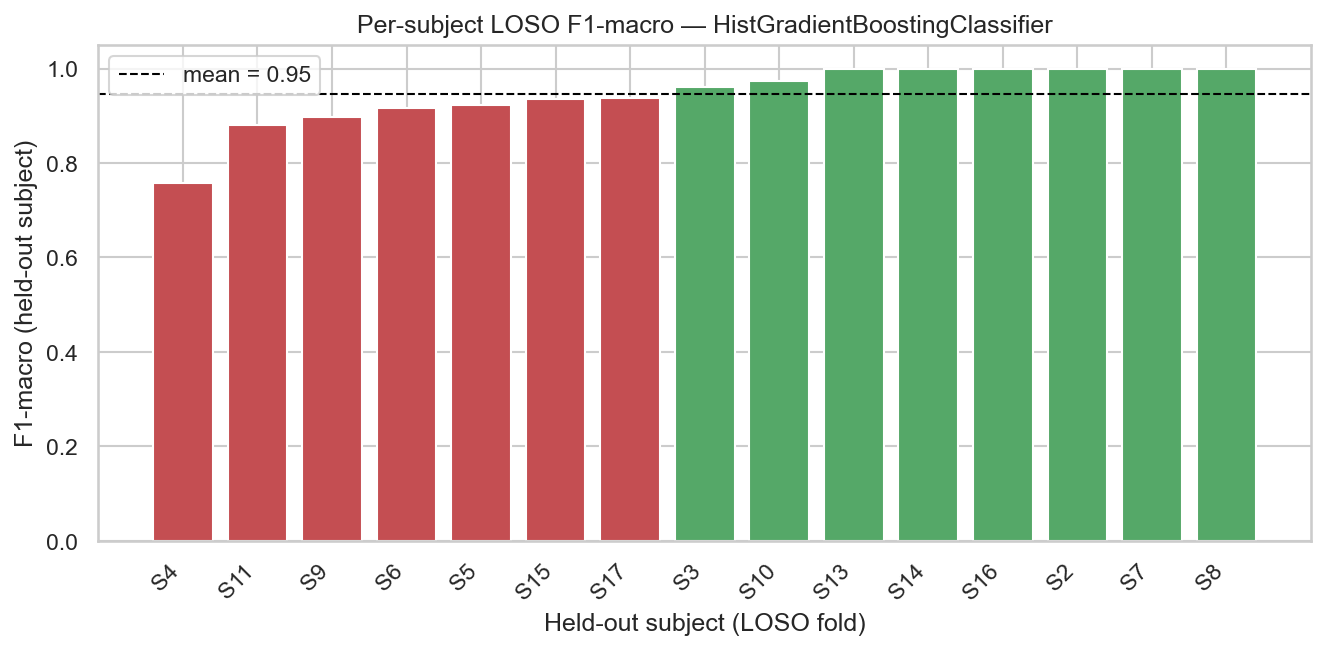
\includegraphics[width=0.48\textwidth]{../results/figures/loso_per_subject_f1.png}
    \hfill
    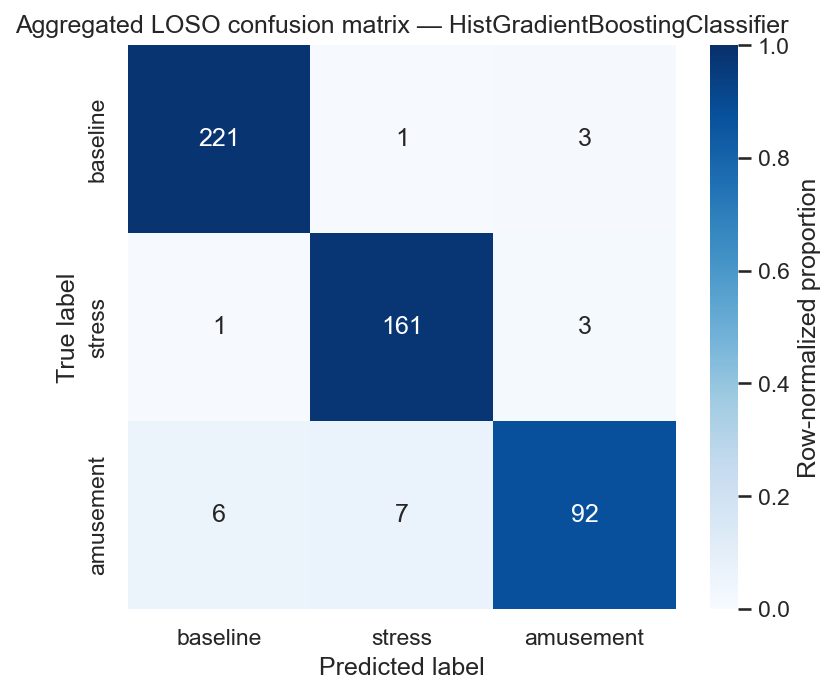
\includegraphics[width=0.48\textwidth]{../results/figures/loso_confusion_matrix.png}
    \caption{معیار اف-یک به ازای هر سوژه و ماتریس درهم‌ریختگی (نوت‌بوک ۰۳)}
\end{figure}

دلیل این امر آن است که تخمین ویژگی‌های پایه هر شخص از نمونه‌های کمی (حدود ۱۵ پنجره) به دست می‌آید و نویز این تخمین بیشتر از مزایای حذف تفاوت‌های فردی است. این یک یافته مهم است: \textbf{استراتژی نرمال‌سازی خود یک انتخاب مدل‌سازی است که باید به‌صورت تجربی ارزیابی شود.}

	\newpage
\section{تفسیرپذیری (\lr{Interpretability})}
اهمیت ویژگی‌ها از طریق سه روش مستقل محاسبه شد:
\begin{enumerate}
    \item \textbf{اهمیت جایگشت (\lr{Permutation Importance}):} محاسبه شده روی سوژه‌های تست و میانگین‌گیری شده در تمام فولدهای \lr{LOSO}.
    \item \textbf{مقادیر شاپلی (\lr{Shapley Values}):} پیاده‌سازی سفارشی از اصول اولیه با استفاده از الگوریتم نمونه‌برداری.
    \item \textbf{آماره \lr{F} در آنالیز واریانس یک‌طرفه (\lr{ANOVA}):} یک بررسی مستقل و فارغ از نوع مدل.
\end{enumerate}

\subsection{ویژگی‌های برتر و سهم هر مدالیته}

\begin{figure}[htbp]
    \centering
    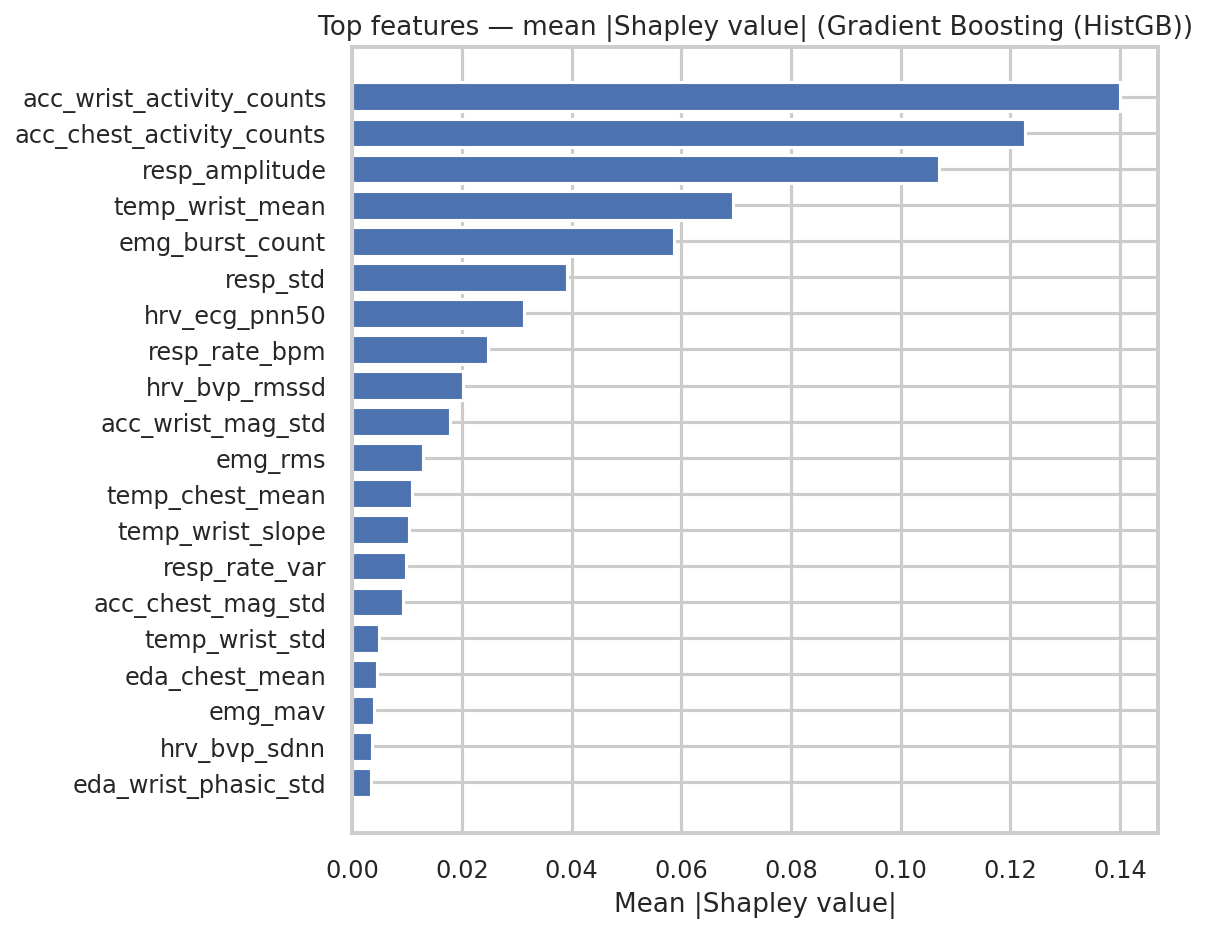
\includegraphics[width=0.8\textwidth]{../results/figures/feature_importance_shap.png}
    \caption{اهمیت ویژگی‌ها بر اساس مقادیر \lr{SHAP}}
\end{figure}

\begin{figure}[htbp]
    \centering
    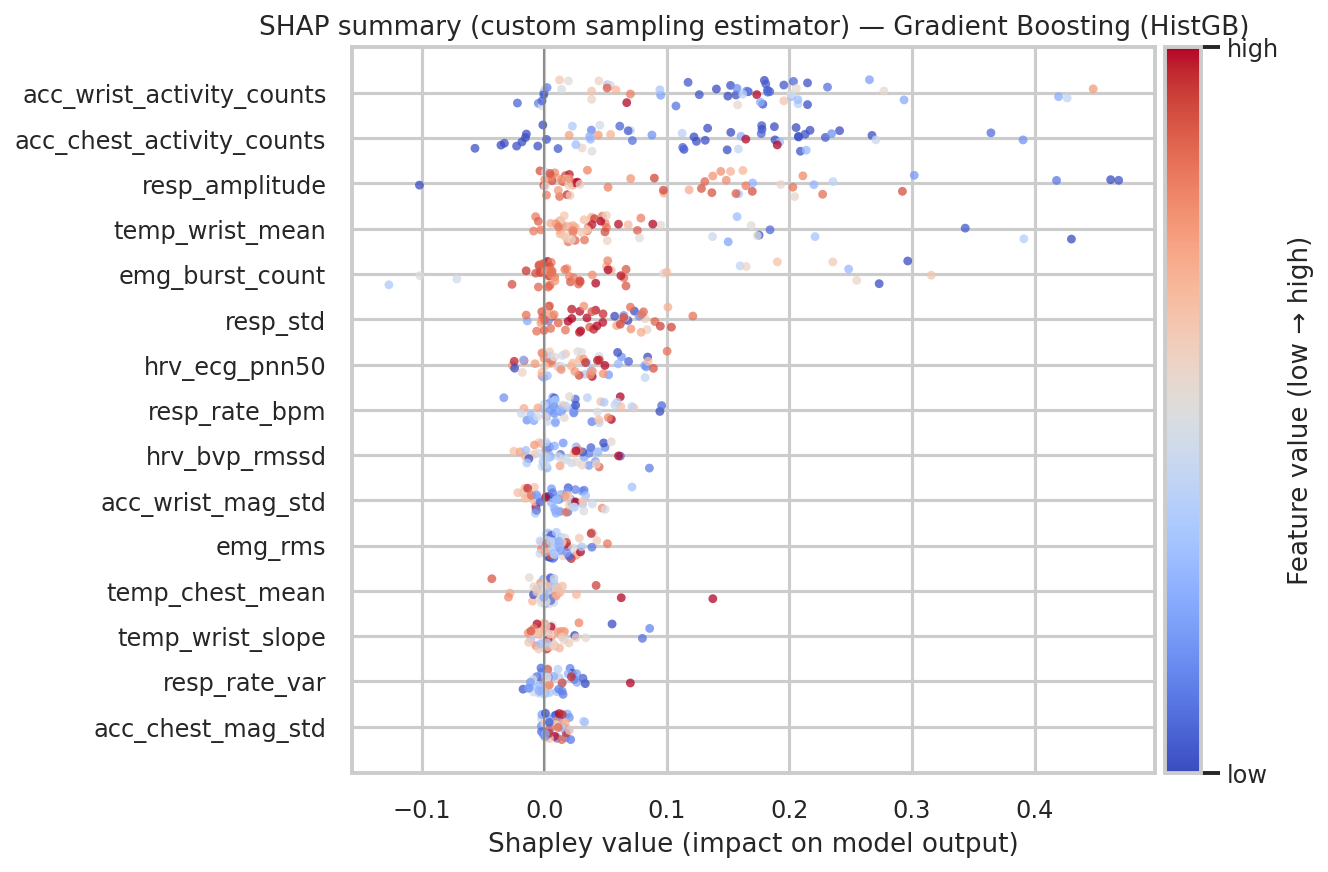
\includegraphics[width=0.8\textwidth]{../results/figures/shap_summary_beeswarm.png}
    \caption{نمودار خلاصه زنبوری \lr{SHAP}}
\end{figure}

\begin{figure}[htbp]
    \centering
    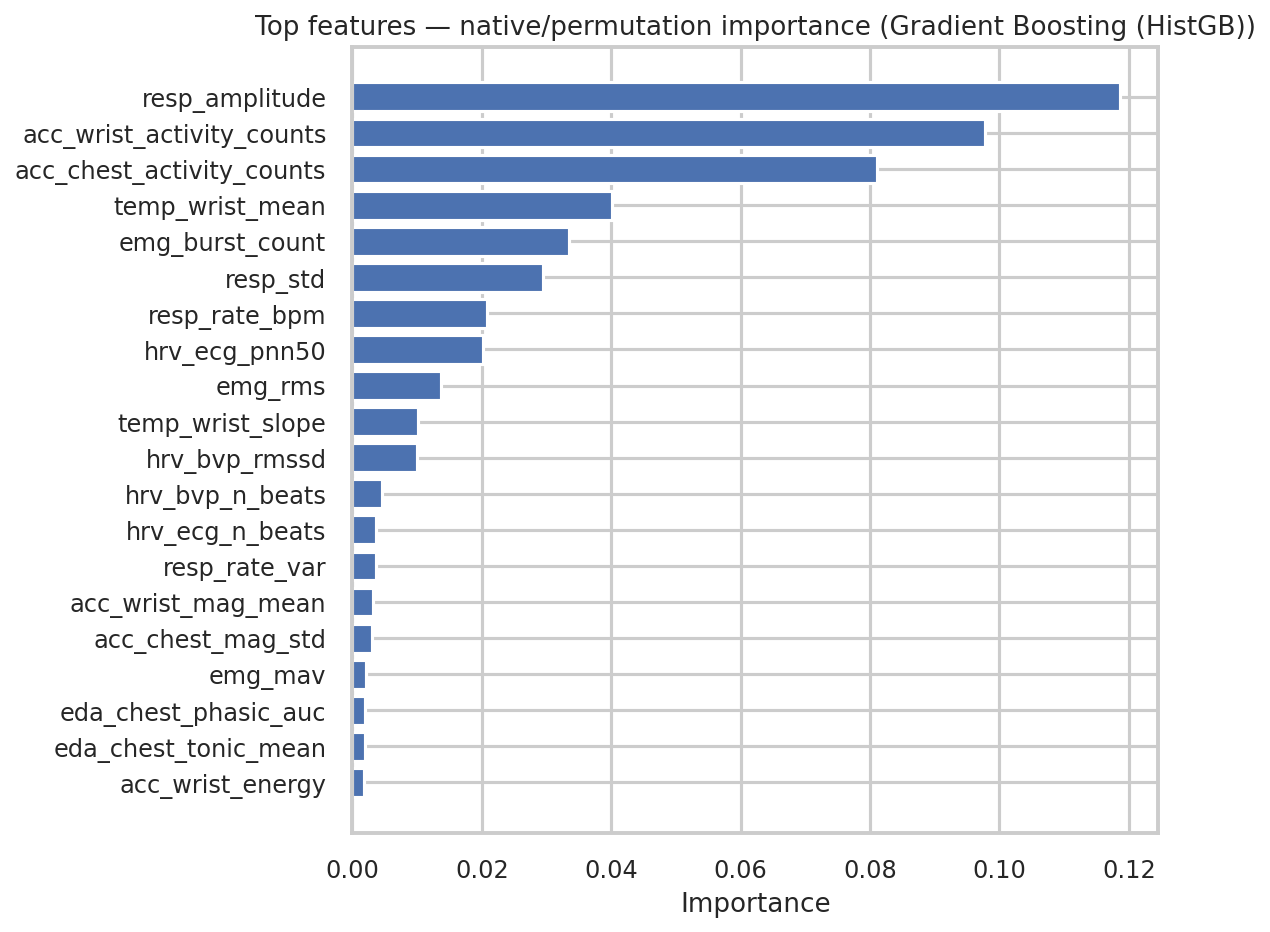
\includegraphics[width=0.8\textwidth]{../results/figures/feature_importance_native.png}
    \caption{اهمیت ویژگی‌ها بر اساس جایگشت (\lr{Native})}
\end{figure}

هر دو روش (شاپلی و جایگشت) روی ۵ ویژگی برتر اتفاق نظر دارند.

\subsection{سهم هر مدالیته سیگنال}

\begin{figure}[htbp]
    \centering
    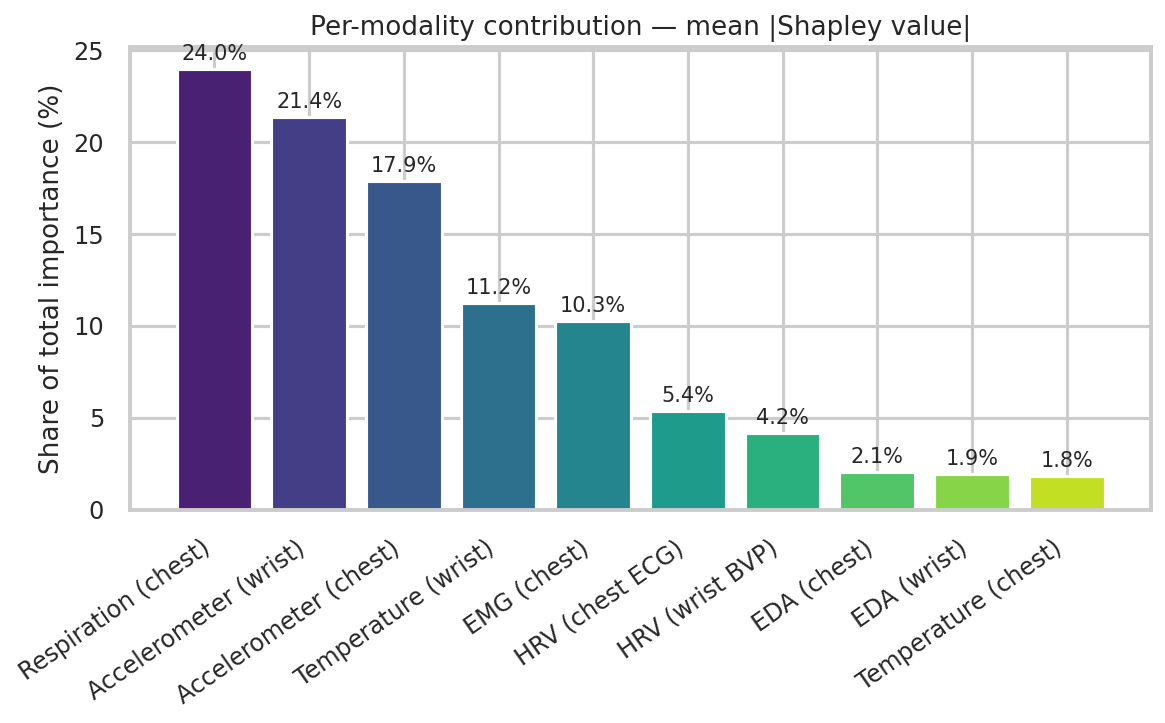
\includegraphics[width=0.8\textwidth]{../results/figures/modality_importance_shap.png}
    \caption{اهمیت هر مدالیته بر اساس \lr{SHAP}}
\end{figure}

\begin{figure}[htbp]
    \centering
    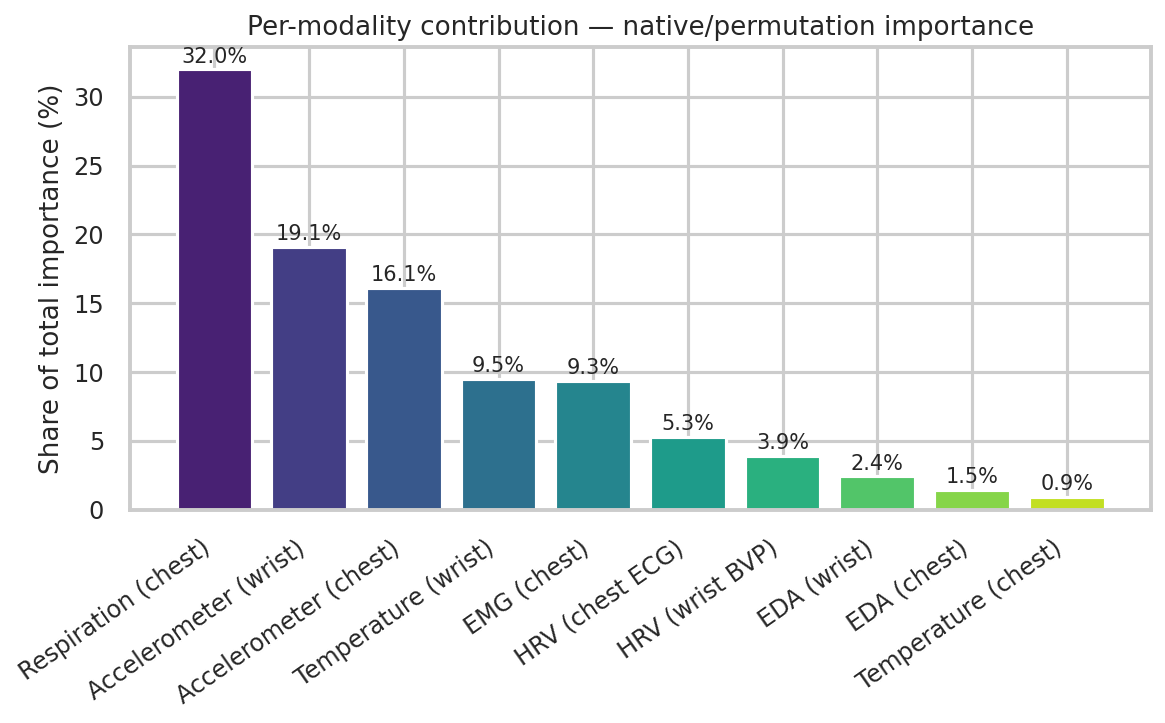
\includegraphics[width=0.8\textwidth]{../results/figures/modality_importance_native.png}
    \caption{اهمیت هر مدالیته بر اساس \lr{Permutation}}
\end{figure}

\begin{figure}[htbp]
    \centering
    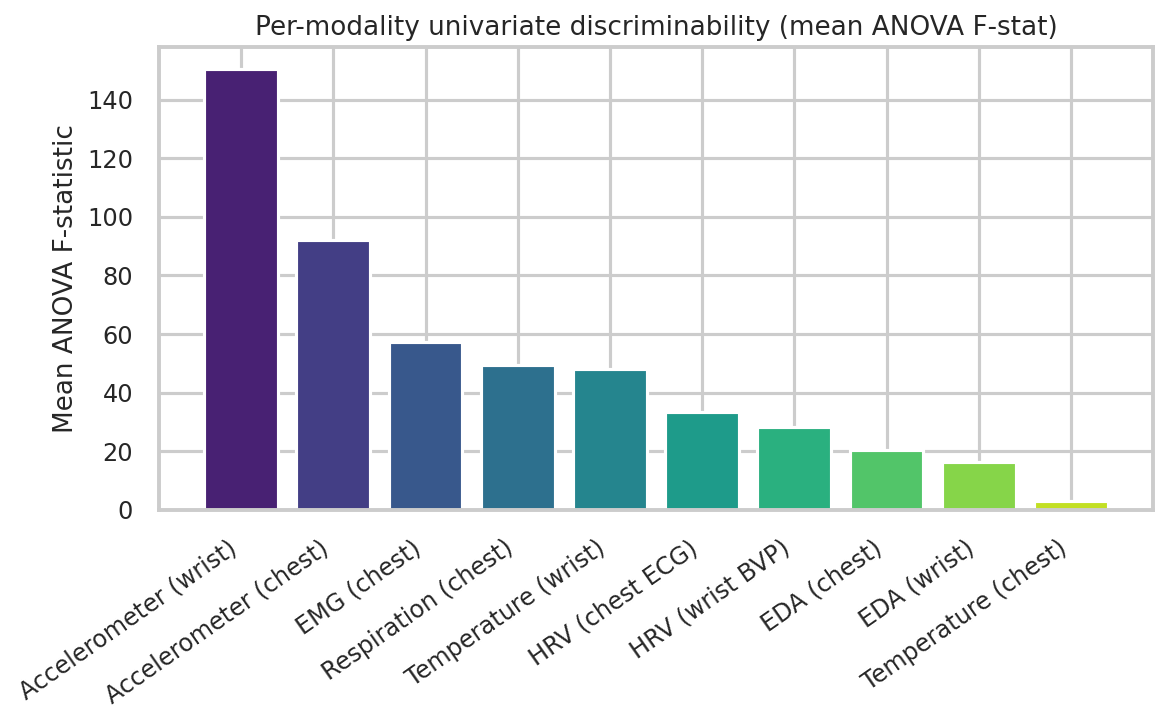
\includegraphics[width=0.8\textwidth]{../results/figures/modality_importance_univariate.png}
    \caption{اهمیت هر مدالیته بر اساس روش \lr{Univariate}}
\end{figure}

\textbf{تفسیر به زبان ساده:} تنفس و حرکت غالب هستند. کم‌عمق شدن تنفس سریع‌ترین نشانه فعال شدن سیستم سمپاتیک است. میزان فعالیت شتاب‌سنج‌ها نیز اهمیت بالایی دارد زیرا بدن در استرس بی‌قرار است، در سرگرمی می‌خندد و تکان می‌خورد، و در حالت پایه بی‌حرکت است. کاهش دمای مچ دست و افزایش انقباض عضلانی نیز از نشانه‌های کلاسیک استرس هستند.

\textbf{چرا \lr{EDA} در صدر نیست؟} اولاً به دلیل افزونگی داده‌ها (وقتی مدل تغییرات تنفس و حرکت را یاد می‌گیرد، اطلاعات جدید ارائه‌شده توسط \lr{EDA} حاشیه‌ای و کمتر خواهد بود). دوماً این نتیجه مختص به مجموعه ویژگی‌های تعریف شده در این پروژه است.

	\newpage
\section{بحث (\lr{Discussion})}

\subsection{آنچه موفقیت‌آمیز بود}
\begin{itemize}
    \item پروتکل \lr{LOSO} به همراه استراتژی‌های نرمال‌سازی منجر به مدلی شد که به خوبی روی افراد جدید تعمیم می‌یابد (دقت ۰.۸۹۱ در برابر خط پایه ۰.۴۵۵).
    \item تمامی سه روش تفسیرپذیری روی مجموعه‌ای مشترک از ویژگی‌های برتر اتفاق نظر داشتند.
    \item پیاده‌سازی مستقل تأیید کرد که دو مدالیته تنفس و حرکت غالب‌ترین شاخص‌ها هستند.
\end{itemize}

\subsection{آنچه کمتر موفق بود و تحلیل خطا}
\begin{itemize}
    \item \textbf{مرز بین استرس و سرگرمی همچنان دشوار است:} ۳۹ خطای دسته‌بندی بین این دو کلاس از مجموع ۴۴ خطا گواه این مدعاست. تمایز این دو حالت با برانگیختگی بالا نیازمند توجه به ابعاد \textit{ظرفیت عاطفی (\lr{Valence})} است که سیگنال‌های محیطی در سنجش آن ضعیف هستند.
    \item \textbf{تفاوت در تعمیم‌پذیری افراد:} دلیل افت دقت روی برخی سوژه‌ها (مثل \lr{S17}) این است که "واکنش‌پذیری" فیزیکی بدن آن‌ها در برابر استرس (در فاکتورهایی مثل تنفس و عضله) نسبت به میانگین جامعه پایین‌تر است.
\end{itemize}


\section{مراجع (\lr{References})}
\begin{itemize}
    \item \lr{Štrumbelj, E., \& Kononenko, I. (2010). An Efficient Explanation of Individual Classifications using Game Theory. \textit{Journal of Machine Learning Research}, 11, 1–18.}
    \item \lr{Lundberg, S. M., \& Lee, S.-I. (2017). A Unified Approach to Interpreting Model Predictions. \textit{Advances in Neural Information Processing Systems} (NeurIPS 2017).}
    \item \lr{Pedregosa, F., et al. (2011). Scikit-learn: Machine Learning in Python. \textit{Journal of Machine Learning Research}, 12, 2825–2830.}
    \item \lr{Virtanen, P., et al. (2020). SciPy 1.0: Fundamental Algorithms for Scientific Computing in Python. \textit{Nature Methods}, 17, 261–272.}
    \item \lr{Harris, C. R., et al. (2020). Array Programming with NumPy. \textit{Nature}, 585, 357–362.}
    \item \lr{McKinney, W. (2010). Data Structures for Statistical Computing in Python. \textit{Proceedings of the 9th Python in Science Conference.}}
\end{itemize}

\end{document}
